%!Cau!%
\begin{ex}%[Tập huấn, Sở GD và ĐT lần 1, 2019]%[Lê Xuân Hòa, 12EX5]%[1D1B2-1]
Nghiệm của phương  trình $\sin 3x = \cos x$ là
\choice
{$x=\pm\dfrac{\pi}{4}+k2\pi,\, k\in\mathbb{Z}$}
{$x=\dfrac{\pi}{4}-k\pi,\, k\in\mathbb{Z}$}
{\True $x=\dfrac{\pi}{4}+k\pi ,x=\dfrac{\pi}{8}+\dfrac{k\pi}{2},\, k\in\mathbb{Z}$}
{$x=\dfrac{\pi}{8}+k\pi, k\in\mathbb{Z}$}
\loigiai{
Ta có
$\sin 3x = \cos x \Leftrightarrow \sin 3x = \sin\left(\dfrac{\pi}{2}-x\right) \Leftrightarrow \hoac{&x=\dfrac{\pi}{8}+\dfrac{k\pi}{2}\\&x=\dfrac{\pi}{4}+k\pi},k\in\mathbb{Z}.$}
\end{ex}%!Cau!%
\begin{ex}%[HK2, THPT Nguyễn Huệ, Vĩnh Phúc, 2019]%[Thịnh Trần, dự án(12EX-5-2019)]%[1D1B2-1]
	Nghiệm của phương trình $\dfrac{1}{2}\sin x\cdot\cos x = 0$ là
	\choice
	{$x = k\dfrac{\pi}{3}$, $k\in\mathbb{Z}$}
	{$x = k\pi$, $k\in\mathbb{Z}$}
	{$x = 2k\pi$, $k\in\mathbb{Z}$}
	{\True $x = k\dfrac{\pi}{2}$, $k\in\mathbb{Z}$}
	\loigiai{
	Ta có	$\dfrac{1}{2}\sin x\cdot\cos x = 0\Leftrightarrow \dfrac{1}{4}\sin 2x=0\Leftrightarrow\sin 2x=0\Leftrightarrow x=k\dfrac{\pi}{2},\, k\in\mathbb{Z}$.
	}
\end{ex}%!Cau!%
\begin{ex}%[Thi tập huấn, Sở GD và ĐT - Bắc Ninh, 2019]%[Nguyễn Minh Tiến, 12EX5]%[1D1B2-1]
	Nghiệm của phương trình $\sin 3x = \cos x$ là
	\choice
	{$x = \pm \dfrac{\pi}{4} + k2\pi; k \in \mathbb{Z}$}
	{$x = \dfrac{\pi}{4} - k\pi; k \in \mathbb{Z}$}
	{\True $x = \dfrac{\pi}{8} + \dfrac{k\pi}{2},x = \dfrac{\pi}{4} + k\pi; k \in \mathbb{Z}$}
	{$x = \dfrac{\pi}{8} + k\pi; k \in \mathbb{Z}$}
	\loigiai{
		\begin{center}
$\sin 3x = \cos x \Leftrightarrow \sin 3x = \sin \left(\dfrac{\pi}{2} - x\right) \Leftrightarrow \hoac{&3x = \dfrac{\pi}{2} - x + k2\pi\\&3x = \dfrac{\pi}{2} + x + k2\pi} \Leftrightarrow \hoac{&x = \dfrac{\pi}{8} + \dfrac{k\pi}{2}\\&x = \dfrac{\pi}{4} + k\pi}; k \in \mathbb{Z}.$
\end{center}
	}
\end{ex}%!Cau!%
\begin{ex}%[Thi thử, Sở GD và ĐT - Hà Tĩnh, 2019]%[Đặng Tân Hoài, 12-EX-5-2019]%[1D1B2-1]
	Phương trình $\cos x=0$ có bao nhiêu nghiệm thuộc khoảng $(-\pi;\pi)$?
	\choice
	{$1$}
	{$3$}
	{\True $2$}
	{$4$}
	\loigiai{
	Ta có $\cos x=0 \Leftrightarrow x=\dfrac{\pi}{2}+k\pi,~k \in \mathbb{Z}$.\\
	Mặt khác $x \in (-\pi;\pi) \Leftrightarrow -\pi <\dfrac{\pi}{2}+k\pi <\pi \Leftrightarrow-\dfrac{3}{2}<k<\dfrac{1}{2}$.\\
	Kết hợp $k \in \mathbb{Z}$ ta được $k \in \{-1;0\}$.\\
	Vậy phương trình đã cho có $2$ nghiệm thuộc khoảng $(-\pi;\pi)$.
	}
\end{ex}%!Cau!%
\begin{ex}%[TT, Hội 8 trường chuyên - Khu vực đông bằng sông Hồng, 2019-L2]%[ Nguyễn Quang Dũng, dự án 12-EX-7-2019]%[1D1B2-1]
Số nghiệm của phương trình $\sin x=0$ trên đoạn $[0;\pi]$ là
\choice
{$1$}
{\True $2$}
{$0$}
{Vô số}
\loigiai{
Ta có $\sin x=0\Leftrightarrow x=k\pi,(k\in\mathbb{Z})$.\\
Do $x\in[0;\pi]\Rightarrow 0\le k\pi\le \pi\Leftrightarrow k\in\{0;1\}$.\\
Suy ra phương trình đã cho có hai nghiệm thuộc đoạn $[0;\pi]$ là $x=0,x=\pi$.}
\end{ex}%!Cau!%
\begin{ex}%[Thi thử L1, Chuyên Lương Thế Vinh Đồng Nai, 2019]%[Nguyễn Tất Thu, dự án(12EX-7)]%[1D1B2-1]
	Phương trình $2\sin x-1=0$ có tập nghiệm là
	\choice
	{\True $S=\left\{\dfrac{\pi}{6}+k2\pi; \dfrac{5\pi}{6}+k2\pi, k\in \mathbb{Z}\right\}$}
	{$S=\left\{\dfrac{\pi}{3}+k2\pi; -\dfrac{2\pi}{3}+k2\pi, k\in \mathbb{Z}\right\}$}
	{$S=\left\{\dfrac{\pi}{6}+k2\pi; -\dfrac{\pi}{6}+k2\pi, k\in \mathbb{Z}\right\}$}
	{$S=\left\{\dfrac{1}{2}+k2\pi, k\in \mathbb{Z}\right\}$}
	\loigiai{
		Giải phương trình $2\sin x-1=0\Leftrightarrow \sin x=\dfrac{1}{2}\Leftrightarrow \hoac{&x=\dfrac{\pi}{6}+k2\pi\\&x=\dfrac{5\pi}{6}+k2\pi},k\in \mathbb{Z}$.
	}
\end{ex}%!Cau!%
\begin{ex}%[Thi thử, Sở GD và ĐT - Hưng Yên-Lần 1, 2019]%[Duong Xuan Loi, 12-EX-8]%[1D1B2-1]
	Phương trình $\sin x-\cos x=1$ có một nghiệm là
	\choice
	{$-\dfrac{\pi}{2}$}
	{\True $\pi $}
	{$\dfrac{\pi}{4}$}
	{$\dfrac{2\pi}{3}$}
	\loigiai{
		Ta có 
		\begin{eqnarray*}
			&& \sin x-\cos x=1 \Leftrightarrow \sin \left(x-\dfrac{\pi}{4}\right)=\dfrac{1}{\sqrt{2}} \\
			&\Leftrightarrow &
			\hoac{& x-\dfrac{\pi}{4}=\dfrac{\pi}{4}+k2\pi \\& x-\dfrac{\pi}{4}=\pi -\dfrac{\pi}{4}+k2\pi} \Leftrightarrow 
			\hoac{& x=\dfrac{\pi}{2}+k2\pi \\	& x=\pi +k2\pi}(k\in\mathbb{R}).
		\end{eqnarray*}		
		Vậy phương trình đã cho có một nghiệm là $x=\pi $.
	}
\end{ex}%!Cau!%
\begin{ex}%[Thi thử L2, Đoàn Thượng  Hải Dương, 2019]%[Nguyễn Tất Thu, dự án EX8]%[1D1B2-1]%Câu 31
	Điều kiện của tham số $m$ để phương trình $m \cdot \sin x-3\cos x=5$ có nghiệm là
	\choice
	{\True $\hoac{
			&m \leqslant -4\\
			&m \geqslant 4\\
		} $}
	{$m \geqslant 4$}
	{$m \geqslant \sqrt{34}$}
	{$-4 \leqslant m \leqslant 4$}
	\loigiai{
		 Phương trình $m \cdot \sin x-3\cos x=5$ có nghiệm khi và chỉ khi \[m^2+(-3)^2 \geqslant 5^2 \Leftrightarrow m^2 \geqslant 16 \Leftrightarrow \hoac{
			& m \leqslant -4 \\
			& m \geqslant 4. \\
		}\]}
\end{ex}%!Cau!%
\begin{ex}%[Đề thi thử L2, Liên trường Nghệ An, 2019]%[Nguyễn Đắc Giáp, dự án 12EX8]%[1D1B2-1]
	Số các giá trị nguyên của $m$ để phương trình $2\sin x-m=1$ có nghiệm là
	\choice
	{\True $5$}
	{$10$}
	{$15$}
	{$4$}
	\loigiai{
		Ta có $2\sin x-m=1 \Leftrightarrow \sin x=\dfrac{m+1}{2}\quad(*)$.\\
		Phương trình $(*)$ có nghiệm khi và chỉ khi $ -1 \leqslant \dfrac{m+1}{2} \leqslant 1 \Leftrightarrow -3 \leqslant m \leqslant 1$.\\
		Mà $m \in \mathbb{Z}$ nên $m \in \{-3,-2,-1,0,1\}$.\\
		Vậy có $5$ giá trị nguyên của $m$ để phương trình $2\sin x-m=1$ có nghiệm.
	}
\end{ex}%!Cau!%
\begin{ex}%[2-TT-5- Đề thi tháng 2-2019, Toán 12 trường THPT chuyên Bắc Giang- 2019]%[Nguyễn Thế Anh-EX6]%[1D1B2-1]
	Phương trình $\sin x=\cos x$ có bao nhiêu nghiệm thuộc đoạn $[-\pi;\pi]$?
	\choice
	{$3$}
	{$5$}
	{\True $2$}
	{$4$}
	\loigiai
	{Ta có: $\sin x=\cos x \Leftrightarrow \tan x=1 \Leftrightarrow x=\dfrac{\pi}{4}+k\pi, k\in\mathbb{Z}$.\\
	Từ ràng buộc $-\pi \le \dfrac{\pi}{4}+k\pi \le \pi$ với $k\in \mathbb{Z}$, ta tìm được hai giá trị của $k$ ứng với hai nghiệm thỏa mãn yêu cầu của bài toán là $k=-1$ và $k=0$.
	}
\end{ex}%!Cau!%
\begin{ex}%[Thi thử L2, THPT Hà Huy Tập - Hà Tĩnh, 2019]%[Phan Ngọc Toàn, dự án EX8]%[1D1B2-1]
Phương trình $\sin\left(3x+\dfrac{\pi}{3}\right)=-\dfrac{\sqrt{3}}{2}$ có bao nhiêu nghiệm thuộc khoảng $\left(0;\dfrac{\pi}{2}\right)$?
	\choice
	{$3$}	
	{$4$}	
	{$1$}	
	{\True $2$}
	\loigiai{Ta có $\sin\left(3x+\dfrac{\pi}{3}\right)=-\dfrac{\sqrt{3}}{2}\Leftrightarrow
	\hoac{&3x+\dfrac{\pi}{3}=-\dfrac{\pi}{3}+k2\pi\\&3x+\dfrac{\pi}{3}=\dfrac{4\pi}{3}+k2\pi}\Leftrightarrow \hoac{&x=-\dfrac{2\pi}{9}+k\dfrac{2\pi}{3}\\&x=\dfrac{\pi}{3}+k\dfrac{2\pi}{3}}$, $k\in\mathbb{Z}$.
\begin{itemize}
\item Nếu $x=\dfrac{\pi}{3}+k\dfrac{2\pi}{3}$, $k\in\mathbb{Z}$ thì có $1$ nghiệm $x=\dfrac{\pi}{3}\in \left(0;\dfrac{\pi}{2}\right)$ ứng với $k=0$.
\item Nếu $x=-\dfrac{2\pi}{9}+k\dfrac{2\pi}{3}$, $k\in\mathbb{Z}$ thì có $1$ nghiệm $x=\dfrac{4\pi}{9}\in\left(0;\dfrac{\pi}{2}\right)$ ứng với $k=1$.
\end{itemize}	
}
\end{ex}%!Cau!%
\begin{ex}%[Đề thử sức, THTT đề số 6]%[Nguyễn Trung Kiên, 12-EX-9-2019]%[1D1B2-1]
	\immini
	{Cho hai điểm $A$, $B$ thuộc đồ thị hàm số $y=\sin{x}$ trên đoạn $[0;\pi]$. Các điểm $C$, $D$ thuộc trục $Ox$ thỏa mãn $ABCD$ là hình chữ nhật và $CD=\dfrac{2\pi}{3}$. Độ dài đoạn $BC$ bằng}
	{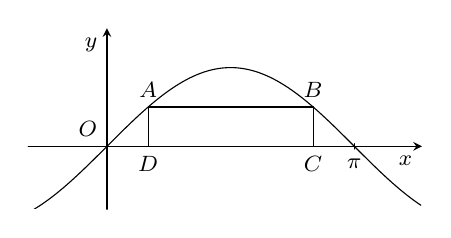
\begin{tikzpicture}[scale=1, font=\footnotesize,line join=round, line cap=round, >=stealth]
		\tikzset{label style/.style={font=\footnotesize}}
		\def \xmin{-1}
		\def \xmax{4}
		\def \ymin{-0.8}
		\def \ymax{1.5}
		\def \hamso{sin(\x r)}
		\draw[->] (\xmin,0)--(\xmax,0) node[below left] {$x$};
		\draw[->] (0,\ymin)--(0,\ymax) node[below left] {$y$};
		\draw (0,0) node [above left] {$O$};
		\draw[thin] (pi,1pt)--(pi,-1pt) node [below] {$\pi$};
		\draw (2.618,0)node[below]{$C$} --(2.618,0.5)node[above]{$B$} --(0.5236,1/2)node[above]{$A$} --(0.5236,0)node[below]{$D$};
		\begin{scope}
		\clip (\xmin+0.01,\ymin+0.01) rectangle (\xmax-0.01,\ymax-0.01);
		\draw[samples=350,domain=\xmin+0.01:\xmax-0.01,smooth,variable=\x] plot (\x,{\hamso});
		\end{scope}
		\end{tikzpicture}}
	\choice
	{$\dfrac{\sqrt{2}}{2}$}
	{\True $\dfrac{1}{2}$}
	{$\dfrac{\sqrt{3}}{2}$}
	{$1$}
	\loigiai
	{Giả sử các điểm $C(c;0)$, $D(d;0)$ với $0<d<c<\pi$. Theo bài ra ta có $CD=c-d=\dfrac{2\pi}{3}\quad(1)$\\
		Khi đó ta có $A\left(d;\sin{d}\right)$, $B\left(c;\sin{c}\right)$. Do $ABCD$ là hình chữ nhật nên 
		$$\sin{c}=\sin{d}\Rightarrow \hoac{&c=d \text{ (loại)}\\&c=\pi-d \text{ (thỏa mãn)}.}$$
		Kết hợp với $(1)$ ta được $\heva{&c-d=\dfrac{2\pi}{3}\\&c+d=\pi}\Leftrightarrow \heva{&c=\dfrac{5\pi}{6}\\&d=\dfrac{\pi}{6}.}$\\
		Vậy $BC=\sin{c}=\sin\dfrac{5\pi}{6}=\dfrac{1}{2}$.}
\end{ex}